% \documentclass[10pt, english, pdftex]{template/UC3M_document}
\documentclass[10pt, spanish, pdftex]{template/UC3M_document}

\usepackage{listings}

%%%%% Preamble %%%%%
\author{Alejandro Prieto Macías}         % This is me! You should write here your name (for PDF metadata)
%%%%% About the authors (will be used on title page and header) %%%%%

%%% Indicate the number of authors by uncommenting the right option.
\authorstwotrue     % 1 or 2 authors
% \authorsthreetrue   % 3 authors
% \authorsfourtrue    % 4 authors

%%% Fill with the authors data. You can leave empty keys {} if you need to and also if you provide more info that number of authors indicated it will be ignored.
% If you selected \authorstwotrue or \authorsthreetrue (1 to 3 authors)
\authorsuptothree{Alejandro Prieto Macías}{NIA 100383428}{Gr. 81}{Laura Sánchez Cerro}{NIA 100383419}{Gr. 81}{Name3 Lastname3}{NIA 100XXXXXX}{Gr. XX}
% If you selected \coauthorsfourtrue (4 authors)
\authorsfour{Name1 Lastname1}{NIA 100XXXXXX}{Name2 Lastname2}{NIA 100XXXXXX}{Name3 Lastname3}{NIA 100XXXXXX}{Name4 Lastname4}{NIA 100XXXXXX}{Group XX}

%%% If you want to show coauthors email address on the title page, uncomment \emailtrue. Comment it otherwise.
% \emailtrue
% You can leave empty keys {} if you need to and also if you provide more info that number of authors indicated or \emailtrue is commented it will be ignored.
\emails{email1@domain.tld}{email2@domain.tld}{email3@domain.tld}{email4@domain.tld}


%%%%% Basic data about the document (Degree, subject, title, campus, page number custom text) %%%%%
\documentdata{Ingeniería Informática}{Sistemas Distribuidos}{Ejercicio Evaluable 1: Colas de mensajes}{Leganés}{ }

%%%%% Page style %%%%%
\header
\footer
\pagestyle{fancy}

\begin{document}
%%%%% Page title %%%%%
\titleMain

%%%%% Index %%%%%
\begin{spacing}{0.5}
    % \shipout\null                   % Blank page before index (after title page)
    \hypersetup{linkcolor=black}    % References/links on the index will remain black color
    \tableofcontents\newpage        % Index of the document
    % \listoffigures\newpage          % Index of pictures
    % \listoftables\newpage           % Index of tables
\end{spacing}


%%%%% Introducción %%%%%
\section{Introducción}\label{section_label}
El motivo de este ejercicio se basa en la idea de poder aprender las técnicas para poder crear una aplicación cliente-servidor de forma concurrente. Además, se pretende aprender a administrar sistema de comunicación para sistemas distribuidos, es decir, para ordenadores que no comparten el espacio de memoria.

  \vspace{2cm}
  \begin{figure}[h]
    \centering
    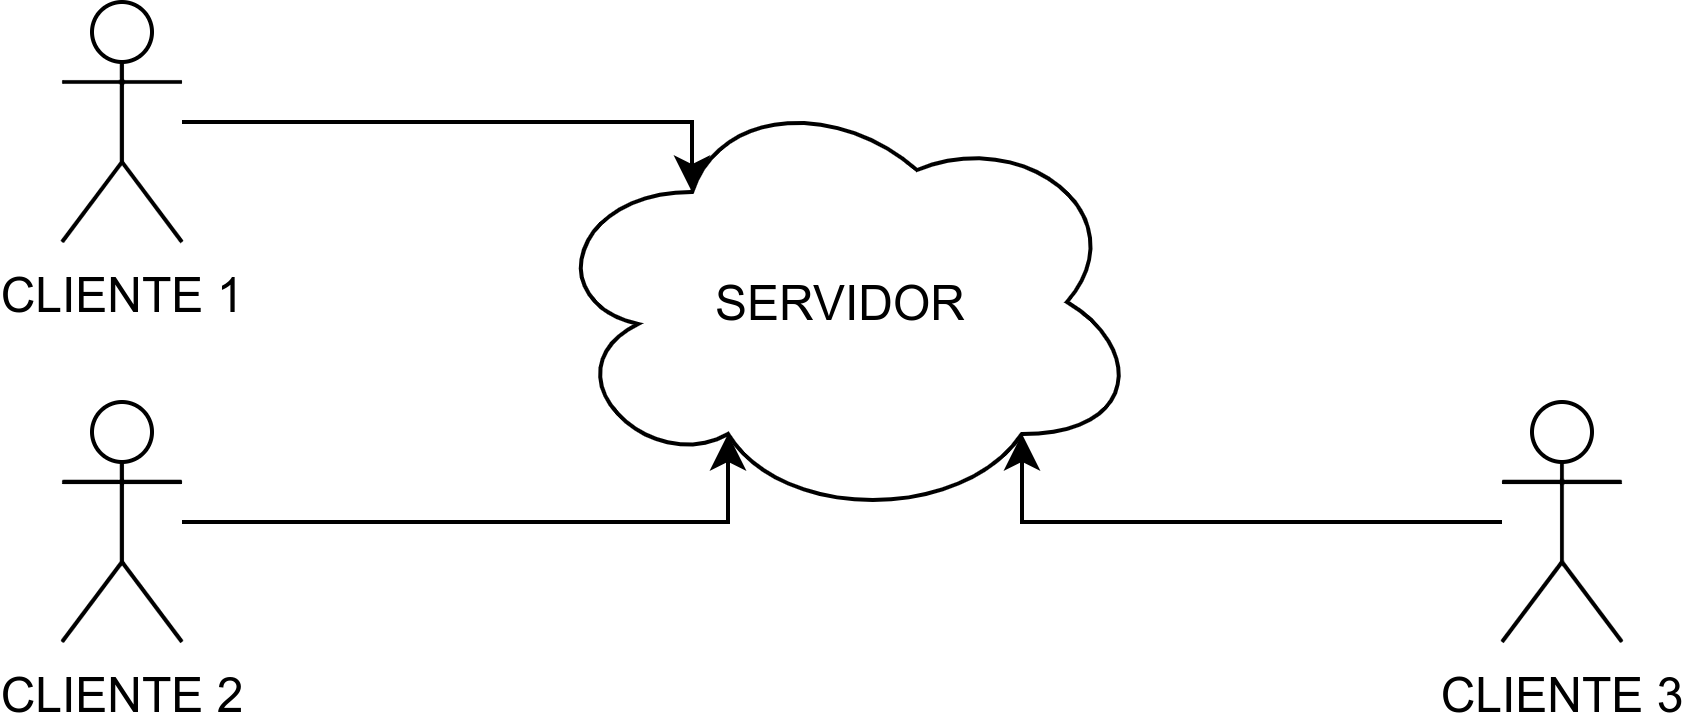
\includegraphics[width=\textwidth]{cliente-servidor.png}
    \caption{Esquema de servicio cliente-servidor concurrente}
  \end{figure}


%%%%Modelo%%%%
\newpage
\section{Modelo}
Este software pretende que el cliente sea capaz de crear vectores de tamaño N, con un nombre, y poder administrarlos a partir de una aplicación. Estos vectores serán almacenados en el servidor con el que se comunica el cliente.

\subsection{Estructura del código}
Los archivos más importantes son cliente.c y servidor.c (bajo demanda) que son las que representan al cliente y al servidor y contienen los respectivos main. En cliente.c se ha añadido unos métodos para imprimir un mensaje con el resultado de las operaciones. Además, se incluyen sus respectivas cabeceras en los archivos cliente.h y servidor.h. El servidor de pool de hilos es el fichero servidorPool.c. El desarrollo de las peticiones del cliente de las operaciones init, get, set y destroy se realizan en los ficheros array.c en la parte cliente y imple.c en la parte servidor.
Para la comunicación entre cliente y servidor hemos creado el fichero comm.h que contiene la estructuras de la petición y la respuesta.

%%%% Compilación %%%%
\subsection{Compilación}
Para poder compilar el ejercicio se puede hacer de forma sencilla con \textit{make all}, esto generará dos tipos de servidores. Uno con la implementación de hilo bajo demanda (\textbf{servidor}) y otro con el pool de hilos (\textbf{servidorPool}). En el caso de que se quiera compilar solo lo necesario, se deberá realizar manualmente haciendo \textit{make} array, cliente, servidor o servidorPool.

Nota: antes de compilar el cliente manualmente, será necesario haber generado la biblioteca dinámica haciendo en primer lugar \textit{make array}.

Para la ejecución del cliente y que no dé problemas con la variable \textit{LD\_LIBRARY\_PATH}, se ha incluido un archivo llamado \textit{cliente.sh} que hará la ejecución para resolver los problemas con la varible mencionada anteriormente.
\subsection{Cliente}
La función del cliente en el sistema es la de utilizar la interfaz gráfica, en este caso el main del archivo \textit{cliente.c} para administrar los datos que el cliente quiere utilizar, es decir, los vectores mencionados anteriormente. Tendrá la capacidades de realizar varias opciones.

\begin{itemize}
  \item \textbf{Crear un vector}: Usará la función \textit{init} para crear el vector especificando el nombre y tamaño a través de los argumentos.
  \item \textbf{Modificar un vector}: Podrá modificar elementos de un vector de tipo número a través de la función \textit{set} indicando la posición en el vector, el nombre del vector y el nuevo valor.
  \item \textbf{Obtener de un vector}: Podrá obtener elementos de tipo número entero del vector a través de la función \textit{get} indicando la posición en el vector, el nombre del vector y la variable valor donde se guardará el dato.
  \item \textbf{Eliminar un vector}: El cliente podrá eliminar con la función \textit{destroy} el vector que desee indicando su nombre.
\end{itemize}

\subsubsection{Biblioteca Dinámica}
En la biblioteca dinámica se han implementado las funciones que se comunicarán con el sistema servidor. La inclusión de estructuras de este estilo facilita la posible mejora de los sistemas de comunicación sin afectar a la interfaz del usuario, incluso pudiendo tener varias interfaces.

\subsection{Servidor}
El servidor será el encargado de recibir las peticiones para que, con ayuda de hilos bajo demanda, se puedan ir ejecutando las acciones que requiere el cliente para administrar los vectores.
El servidor debe estar configurado de tal manera que se evite que se pierdan peticiones debido a condiciones de carrera y, para ello, se emplearán herramientas de POSIX. Hemos optado por implementarlo mediante un cerrojo y una variable condicional que hacen que no se pueda atender a una nueva petición si no se atendió a la anterior. El término "atender" no se refiere a procesar la petición, simplemente al hecho de copiar la petición de entrada en una variable local y evitar que se pierda.

\subsection{Servidor Pool de Hilos}
Se ha implementado también la versión con un pool de hilos que consiste en crear un número de hilos determinados. Cada vez que llega una nueva petición se almacena en una cola circular de tareas y serán los hilos los que se encargan de recoger y procesar esas tareas cuando puedan actuar. Se trata de una versión del problema de \textit{productor-consumidor} en el que produce el hilo principal y los hilos que se crean son los que consumen de la cola circular.


\subsubsection{Modelo de datos}
Para administrar la estructura de datos que almacena los vectores se ha decidido establecer una lista enlazada implementada a través de un \textit{struct} del lenguaje de programación \textbf{C}. Cada elemento de la lista está formado por un vector de enteros de tamaño N, una cadena de caracteres que representa el nombre del vector y un puntero al siguiente elemento.
Además, las peticiones se han podido realizar mediante \textit{structs} debido a la tecnología de comunicación que son las colas de mensajes del sistema UNIX.

\subsubsection{Implementación}
Las funciones que manejan la lista enlazada se encuentran en un archivo distinto al del propio servidor para facilitar los cambios en el sistema, dando prioridad a la modularización del sistema. Las funciones que realizan los clientes tienen su correspondencia en el servidor. Todas ellas devuelven los valores indicados en el enunciado.
\begin{itemize}
    \item \textbf{Crear un vector}: La función \textit{INIT} será la encargada de crear un nuevo elemento en la lista. Para ello, se debe reservar en memoria el tamaño necesario para almacenar un vector de N enteros, la cadena de caracteres (nombre del vector) de tamaño \textbf{MAX} (que se establece en 100 caracteres) y el puntero. Además, se deberá enlazar al final de la lista con el elemento correspondiente.
    \item \textbf{Modificar un vector}: La función \textit{SET} se encargará de encontrar el vector en la lista a través del nombre y, posteriormente, se encargará de cambiar el valor que se almacenaba en la posición indicada por el valor que se desea introducir.
    \item \textbf{Obtener de un vector}: La función \textit{GET} se encargará de encontrar el vector en la lista a través del nombre y, posteriormente, guardará el valor que se almacenaba en la posición indicada en la variable que se pasa como parámetro.
    \item \textbf{Eliminar un vector}: La función \textit{DESTROY} se encarga de eliminar el espacio de memoria que ocupaba el vector en la lista y, además, enlazar correctamente los elementos de lista para evitar que queden elementos sin apuntar.
\end{itemize}

% %%%%Pruebas%%%%
\section{Pruebas}
Para verificar el correcto funcionamiento de las operaciones en el servidor hemos creado el método \textit{show} que muestra la lista con el contenido de todos los vectores para ver las modificaciones.Además, hemos creado unos métodos en el cliente que muestra el resultado de los métodos (ErrorMsgInit, ErrorMsgSet, ErrorMsgGet y ErrorMsgDestroy).

\begin{itemize}
  \item \textbf{init} \\
    Para probar el funcionamiento del método init primero introducimos un vector llamado "vector1" de tamaño 10. La salida en este caso es: 1. Después, introducimos otro vector con el mismo nombre y mismo tamaño. La salida es: 0 y no se enlaza en la lista. Finalmente, introducimos otro vector del mismo nombre y tamaño distinto y la salida es -1. Añadimos otro vector de distinto nombre y tamaño y se añade a la lista sin problemas.

    \begin{figure}[H]
      \centering
      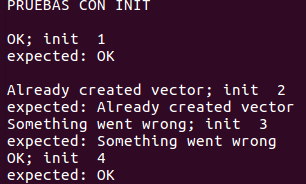
\includegraphics [scale=0.4]{INIT.png}
      \caption{Pruebas de función init}
    \end{figure}

También se ha probado a crear un vector con un nombre y una dimensión desde un cliente e intentar volver a crearlo igual desde otro cliente. Se comprueba que el primero lo crea correctamente, pero al segundo cliente le da un mensaje de que el vector ya existe.
    \begin{figure}[H]
      \centering
      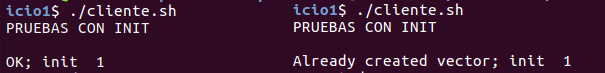
\includegraphics [scale=0.4]{INIT2clientes.png}
      \caption{Pruebas de función init}
    \end{figure}

  \item \textbf{set}\\
    Modificamos el valor de un vector que está en la lista y en una posición correcta, la salida es 0. Después, modificamos el valor de un vector cuyo nombre no se encuentra en la lista, la salida es -1 . Finalmente, intentamos modificar el valor de una posición de un vector de la lista fuera de rango (de tamaño mayor del vector), la salida es -1.

    \begin{figure}[H]
      \centering
      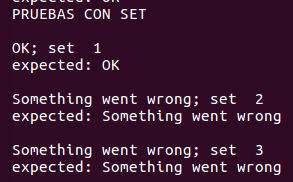
\includegraphics [scale=0.4]{SET.png}
      \caption{Pruebas de función set}
    \end{figure}

 \item \textbf{get}\\
  Obtenemos el valor de un vector que está en la lista y en una posición correcta, la salida es 0. Después, obtenemos el valor de un vector cuyo nombre no se encuentra en la lista, la salida es -1 . Finalmente, intentamos obtener el valor de una posición de un vector de la lista fuera de rango (de tamaño mayor del vector), la salida es -1.

  \begin{figure}[H]
    \centering
    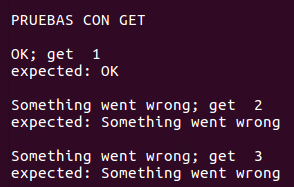
\includegraphics [scale=0.4]{GET.png}
    \caption{Pruebas de función get}
  \end{figure}

 \item \textbf{destroy}\\
    Eliminamos un vector que está en la lista, la salida es 1. Después, eliminamos un vector cuyo nombre no se encuentra en la lista, la salida es -1 . Finalmente, se prueba que se borra correctamente un vector situado en mitad de la lista, al principio de la lista y al final de la lista con el fin de observar que se hacen correctamente los enlaces.

    \begin{figure}[H]
      \centering
      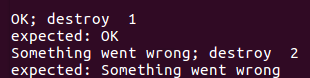
\includegraphics [scale=0.4]{DESTROY.png}
      \caption{Pruebas de función destroy}
    \end{figure}

\end{itemize}


\newpage


%%%% Conclusiones %%%%
\section{Conclusiones}
Esta práctica nos ha permitido aprender la estructura básica de un sistema de tipo cliente-servidor, pudiendo descubrir algunas de sus ventajas y desventajas.

\begin{itemize}
  \item \textbf{Ventajas}
    \begin{itemize}
      \item Modularidad.
      \item Menor cómputo en los dispositivos de los clientes.
    \end{itemize}
  \item \textbf{Desventajas}
  \begin{itemize}
    \item Mucha dependencia de los servidores.
    \item Puede llegar a colapsar el sevicio si llegan demasiadas peticiones.
  \end{itemize}
\end{itemize}

Por otro lado, hemos tenido ciertas dificultades a la hora de realizar la concurrencia puesto que en la implementación con hilos \textit{bajo demanda} se lanzan muchos más hilos llegando incluso a poder empeorar la calidad del servicio, mientras que con una implementación de \textit{pool de hilos} el sistema es mucho más eficaz. Decidimos empezar la tarea con \textit{hilos bajo demanda} y resultó menos complejo, tras completar esta versión pudimos realizar la versión con el \textit{pool de hilos}.


\end{document}
